Given, 
\begin{align}
\vec{p} = \myvec{4\\3} , \vec{q} = \myvec{ 6\\2}
\end{align}
are the points on the ellipse.
The general form of the conic is given by
\begin{align}
\label{quadform/72/k/eq:2}
\vec{x}^{\top}\vec{D}\vec{x} = 1, \quad \vec{D} = \myvec{\lambda_1 & 0 \\ 0 & \lambda_2}, \lambda_1,\lambda_2 > 0
\end{align}
The points $\vec{p}$ and $\vec{q}$ satisfy \eqref{quadform/72/k/eq:2}, and thus we have
\begin{align}
\label{quadform/72/k/eq:ellipse_std_ab}
\vec{p}^{\top}\vec{D}\vec{p} &= 1,
\\
\vec{q}^{\top}\vec{D}\vec{q} &= 1
\end{align}
which can be further expressed as,
\begin{align}
\label{quadform/72/k/eq:5}
\begin{split}
\vec{p}^{\top}\vec{P}\vec{d} &= 1,
\\
\vec{q}^{\top}\vec{Q}\vec{d} &= 1
\end{split}
\end{align}
where,
\begin{align}
\vec{d} = \myvec{\lambda_1\\ \lambda_2},
\vec{P} = \myvec{4 & 0 \\ 0 & 3},
\vec{Q} = \myvec{6 & 0 \\ 0 & 2}.
\end{align}
\eqref{quadform/72/k/eq:5} can then be expressed as,
\begin{align}
\myvec{\vec{p}^{\top}\vec{P}\\ \vec{q}^{\top}\vec{Q}}\vec{d} &= \myvec{1\\1}\\
\myvec{16 & 9\\ 36 & 4}\vec{d} &= \myvec{1\\1}\label{quadform/72/k/eq:8}
\end{align}
The augmented matrix is 
\begin{align}
\myvec{16 & 9 & 1 \\ 36 & 4 & 1 }
\end{align}
and we perform row reduction,
\begin{align}
\myvec{16 & 9 & 1\\ 1 & 16 & 1} 
\xleftrightarrow{R_1\rightarrow \frac{R_1}{16}}
\myvec{1 & \frac{9}{16} & \frac{1}{16} \\ 36 & 4 & 1} 
\\
\xleftrightarrow{R_2\rightarrow R_2-36R_1}
\myvec{1 & \frac{9}{16} & \frac{1}{16} \\ 0 & \frac{-65}{4} & \frac{-5}{4}} 
\\
\xleftrightarrow{R_2\rightarrow \frac{-4}{65}R_2}
\myvec{1 & \frac{9}{16} & \frac{1}{16} \\ 0 & 1 & \frac{1}{13}}
\\
\xleftrightarrow{R_1\rightarrow R_1-\frac{9}{16}R_2}
\myvec{1 & 0 & \frac{1}{52} \\ 0 & 1 & \frac{1}{13}}
\\
\implies \vec{d} = \myvec{\frac{1}{52} \\ \frac{1}{13}}.
\end{align}
Thus we have,
\begin{align}
    \vec{D} = \myvec{\frac{1}{52} & 0 \\ 0 & \frac{1}{13}}
\end{align}
Hence equation of ellipse is given by,
\begin{align}
\vec{x}^{\top}\myvec{\frac{1}{52} & 0 \\ 0 & \frac{1}{13}}\vec{x} = 1
\end{align}
The plot of the ellipse is given below
\numberwithin{figure}{section}
\begin{figure}[ht]
\centering
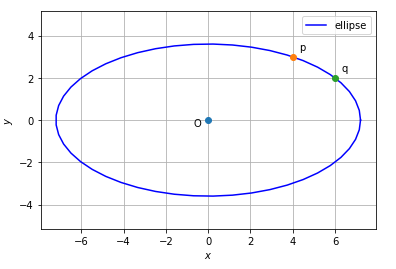
\includegraphics[width=\columnwidth]{solutions/su2021/2/72/k/ellipse(1).PNG}
\caption{Plot of standard ellipse}
\label{quadform/72/k/Plot of standard ellipse}
\end{figure}
The center and axes of the ellipse is given as
\begin{align}
\vec{c} = \vec{0};
\frac{1}{\sqrt{\lambda_1}}  = \sqrt{52},
\frac{1}{\sqrt{\lambda_2}} =\sqrt{13}.
\end{align}
Now let us consider the case when the ellipse is not in the standard form then we have the center to be $\vec{c}=\myvec{\beta\\0}$.The equation is given by:
\begin{align}
(\vec{x}-\vec{c})^{\top}\vec{D}(\vec{x}-\vec{c})=1\label{quadform/72/k/eq:14}
\end{align}
where $\vec{D}$ is a diagonal matrix.
$\because \vec{p}, \vec{q}$ satisfy \eqref{quadform/72/k/eq:14}, we have
\begin{align}
\label{quadform/72/k/eq:ellipse_act_ab}
(\vec{p}-\vec{c})^{\top}\vec{D}(\vec{p}-\vec{c}) &= 1,
\\
(\vec{q}-\vec{c})^{\top}\vec{D}(\vec{q}-\vec{c}) &= 1,
\end{align}
which can be simplified as
\begin{align}
    2\brak{\vec{p}-\vec{q}}^{\top}\vec{D}\vec{c}=\vec{p}^{\top}\vec{D}\vec{p}-\vec{q}^{\top}\vec{D}\vec{q} \label{quadform/72/k/eq:4}
\end{align}
Using the identity,
\begin{align}
   (\vec{p}^{\top}-\vec{q}^{\top})\vec{D}(\vec{p}+\vec{q})
   =\vec{p}^{\top}\vec{D}\vec{p}-\vec{q}^{\top}\vec{D}\vec{q}
\end{align}
in the equation \eqref{quadform/72/k/eq:4}
\begin{align}
    2\brak{\vec{p}-\vec{q}}^{\top}\vec{D}\vec{c}=(\vec{p}-\vec{q})^{\top}\vec{D}(\vec{p}+\vec{q})\\
    \implies (\vec{p}-\vec{q})^{\top}\vec{D}(2\vec{c}-(\vec{p}+\vec{q}))
\end{align}
Thus $\vec{c}$ can be expressed in parametric form as
\begin{align}
\vec{c}=\frac{1}{2}((\vec{p}+\vec{q})+k\vec{D}^{-1}\vec{m}) \label{quadform/72/k/eq:7}
\end{align}
where,
\begin{align}
    (\vec{p}-\vec{q})^{\top}\vec{m}=0 \label{quadform/72/k/eq:6}
\end{align}
and $k$ is a constant.Substituting numerical values in \eqref{quadform/72/k/eq:6}, \begin{align}
    \vec{p}-\vec{q} = \myvec{-2 \\ 1} \implies \vec{m} = \myvec{-1 \\ -2}
\end{align}
and
\begin{align}
    \vec{p}+\vec{q} = \myvec{10 \\ 5}
\end{align}
substituting in \eqref{quadform/72/k/eq:7},we get
\begin{align}
 \myvec{\beta\\0}=\frac{1}{2}\brak{\myvec{10 \\ 5} + k\myvec{\frac{1}{\lambda_1}&0 \\ 0&\frac{1}{\lambda_2}}\myvec{-1 \\ -2}}
\end{align}
From the given information,the X-axis is the major axis.Hence,
\begin{align}
\frac{\lambda_2}{\lambda_1}>1 \implies
    \frac{20-4\beta}{5}>1\\
    \beta<3.75
\end{align}
The possible ellipse satisfying the above conditions are plotted below
\begin{figure}[!ht]
\centering
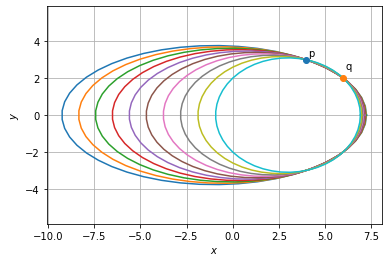
\includegraphics[width=\columnwidth]{solutions/su2021/2/72/k/Ellipse_(I).PNG}
\caption{Ellipses passing through the two points with X axis as major axis}
\label{quadform/72/k/fig:ellipses}	
\end{figure}

